\documentclass[12pt,a4paper]{article}
\usepackage{mathptmx} % added for time new roman font
\usepackage[left=0.5in,right=0.5in,top=1in,bottom=1in]{geometry}
\usepackage[latin1]{inputenc}
\usepackage{amsmath}
\usepackage{amsfonts}
\usepackage{amssymb}
\usepackage{graphicx}
\usepackage{float}
\usepackage{booktabs}
\usepackage{parskip} % remove all the paragraph indents


\usepackage{setspace}
\usepackage[colorlinks=true]{hyperref}
\usepackage{textcomp} 
\usepackage{multicol} 

\usepackage{mathtools}          %loads amsmath as well added for the piece wise function
\DeclarePairedDelimiter\Floor\lfloor\rfloor
\DeclarePairedDelimiter\Ceil\lceil\rceil

 
\newcounter{NumberInTable}
\newcommand{\LTNUM}{\stepcounter{NumberInTable}{(\theNumberInTable)}}

\newcommand{\Laplace}[1]{\ensuremath{\mathcal{L}{\left[#1\right]}}}
\newcommand{\InvLap}[1]{\ensuremath{\mathcal{L}^{-1}{\left[#1\right]}}}
\renewcommand{\textuparrow}{$\uparrow$}

\begin{document}
	
	\large{}
	\title{\vspace{-2cm}Lecture Notes, Topic-10}
	\date{}
	\maketitle
	
	\section*{Review from previous class}
		\begin{enumerate}
			\item Transform Method for deterministic inputs (harmonic, step, impulse)
		\end{enumerate}
	
	\section*{Objectives for today's class}
	\begin{enumerate}
		\item Transform function for response to random inputs
	\end{enumerate}
	
	\section*{Lecture}

\subsection*{Defining the transfer function $\mathbf{H(s)}$}

Again, consider the following system
\begin{figure}[H]
	\centering
	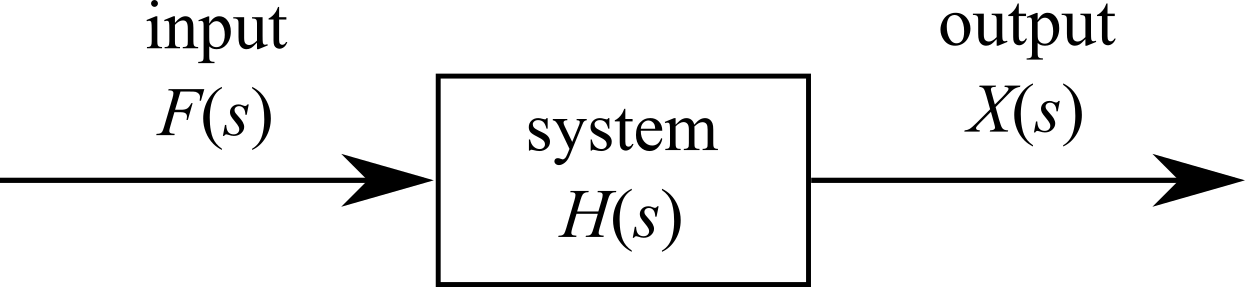
\includegraphics[width=0.5\textwidth]{../../Figures/system_input_output.png}
\end{figure}
For this system representation, F(s) is the Laplace of the transform of the driving force and H(s) is the Laplace transform of the response of the system h(t). 

We need to define transfer function $H(s)$ for a generic system. To do this let us show the reasoning behind the transfer function. \textbf{Here we will show that the output of any system ($x(t)$) can be related to the input of the system ($f(t)$) through a series of polynomial coefficients ($a$ and $b$).} Consider the general $n^{th}$-order linear, time-invariant differential equation that governs the behavior of the dynamic system.

\begin{equation}
a_n\frac{d^nx(t)}{dt^n} + a_{n-1}\frac{d^{n-1}x(t)}{dt^{n-1}} + ... + a_0x(t) = b_m\frac{d^mf(t)}{dt^m} + b_{m-1}\frac{d^{m-1}f(t)}{dt^{m-1}} + ... + b_0f(t)
\end{equation} 
where $x(t)$ is the output and $f(t)$ is the input. Note that this is similar to the formulation we have had before for the EOM. Taking the Laplace transformation of both side of the above equation yields

\begin{eqnarray}
&a_ns^nX(s) + a_{n-1}s^{n-1}X(s) + ... + a_0X(s) + \text{initial condition involving } x(t) =   \\
&b_ms^mF(s) + b_{m-1}s^{m-1}F(s) + ... + b_0F(s) + \text{initial condition involving } f(t)  \nonumber
\end{eqnarray}
It can be seen that this equation is a purely algebraic expression. If we assume the initial conditions to be zero, the equation reduces to the following:
\begin{eqnarray}
(a_ns^n + a_{n-1}s^{n-1} + ... + a_0)X(s) =  (b_ms^m + b_{m-1}s^{m-1} + ... + b_0)F(s) 
\end{eqnarray}
we can rearrange the equation as 
\begin{equation}
H(s) = \frac{X(s)}{F(s)} = \frac{b_ms^m + b_{m-1}s^{m-1} + ... + b_0}{a_ns^n + a_{n-1}s^{n-1} + ... + a_0}
\end{equation}
where H(s) is the \textbf{transfer function} that is defined as:

\textit{The ratio of the Laplace transforms of the output or response function to the laplace transform of the input or forcing function assuming zero initial conditions.}

This can be rearranged to show that the output of the system $X(s)$ can be obtained if we know the input $F(s)$ and the transfer function $H(s)$:
\begin{equation}
X(s) = H(s)F(s)
\end{equation}	


\subsection*{Transfer Function method (Steady-State solution)}

Considering the forced system:
\begin{figure}[H]
	\centering
	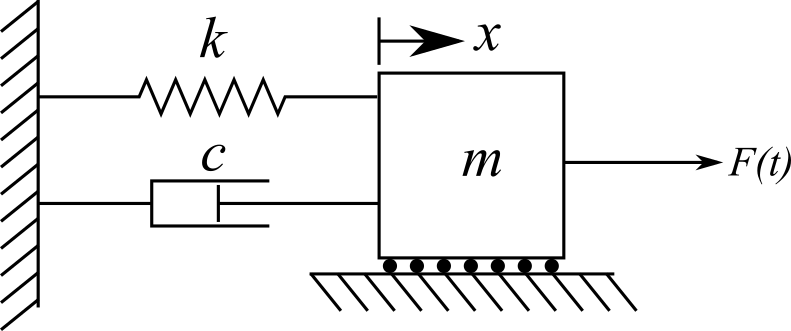
\includegraphics[width=0.4\textwidth]{../../Figures/forced_spring_mass_damper_system.png}
\end{figure}
that can be expressed as the equation of motion
\begin{equation}
	m\ddot{x} + c\dot{x} +kx = F_0 \cos(\omega t)
\end{equation}
Here $F_0 \cos(\omega t)$, is used at the input but any input will develope the same transfer function as the transfer function is bounded to the system and not the input. From the \#6 in the table for Laplace Transforms, we know that
\begin{equation}
	\Laplace{\cos(\omega t)} = \frac{s}{s^2+\omega^2}
\end{equation}
Therefore, 
\begin{equation}
F(s) = \frac{F_0s}{s^2+\omega^2}
\end{equation}
Ignoring the initial conditions, and therefore considering only the partial solution, and taking the Laplace transform of the EOM equation yields:
\begin{equation}
(ms^2 + cs +k)X(s) = \frac{F_0s}{s^2+\omega^2} 
\end{equation}
where $s$ is the complex transform variable and $X(s)$ denotes the Laplace transform of the unknown function x(t). Solving algebraically for the $X(s)$ yields: 
\begin{equation}
X(s) = \frac{F_0s}{(ms^2 + cs +k)(s^2+\omega^2)}
\end{equation}
Now that we have $F(s)$ and $X(s)$ we can obtain $H(s)$ as  
\begin{equation}
H(s) = \frac{X(s)}{F(s)} = \frac{F_0s}{(ms^2 + cs +k)(s^2+\omega^2)} \cdot \frac{s^2+\omega^2}{F_0s} = \frac{1}{ms^2+cs+k}
\end{equation}
or 
\begin{equation}
H(s) = \frac{1}{ms^2+cs+k}
\end{equation}
This ratio is termed the \textbf{transfer function of a system} and is an important tool in vibration analysis.

Recall that $s$ is a complex number, if the value of $s$ is restricted to lie along the imaginary axis in the complex plane (i.e., if $s = j\omega$), the transfer function becomes:
\begin{equation}
H(j\omega) = \frac{1}{m(j\omega)^2+cj\omega+k} = \frac{1}{-m\omega^2+cj\omega+k} 
\end{equation}
rearranging into a standard form yields:
\begin{eqnarray}
H(j\omega) = \frac{1}{k-m\omega^2+c\omega j}
\end{eqnarray}
recall that $j^2=-1$. This is the \textbf{frequency response function of the system}. Therefore, it can bee seen that the frequency response function of the system is the transfer function of the system evaluated along the imaginary axis $s=j\omega$. However, this expression contains imaginary values (that help to account for the phase in the system) and therefore can be challenging to work with. If we ignore the phase component and only consider the amplitude $|H(j\omega)|$ of the response (the real portion of the equation) we get:
\begin{eqnarray}
H(\omega) = |H(j\omega)| = \frac{1}{\sqrt{(k-m\omega^2)^2+c^2\omega^2}}
\end{eqnarray}
where $|H(j\omega)|$ represents only the amplitude of the frequency response function. A more detailed derivation can be found in [Mechanical Vibrations - Rao, 6th edition]



To recap, for a single DOF damped spring-mass system the \textbf{transfer function} is:
\begin{equation}
H(s) = \frac{1}{ms^2+cs+k}
\end{equation}
And the \textbf{frequency response function} is:
\begin{eqnarray}
H(j\omega) = \frac{1}{k-m\omega^2+c\omega j}
\end{eqnarray}
While the amplitude of the frequency response is:
\begin{eqnarray}
H(\omega) = |H(j\omega)| = \frac{1}{\sqrt{(k-m\omega^2)^2+c^2\omega^2}}
\end{eqnarray}




\subsection*{Response to Random Inputs}
The transfer and frequency response functions can be very useful for demeriting the response to random inputs. Up to this point we have solved for deterministic input. 

\begin{itemize}
\item \textbf{Deterministic}-For a known time $t$, the value of the input force $F(t)$ is precisely known. 
\item \textbf{Random} For a known time $t$, the value of the input force $F(t)$ is known only statistically. 
\end{itemize}

To expand, a random signal is a signal with no obvious pattern. For these types of it is not possible to focus on the details of the input signal, as is done with a deterministic signal, rather the signal is classified and manipulated in terms of its statistical properties. 

Randomness in vibration analysis can be thought of as the result of a series of results obtained from testing a system repeatability for various inputs under varying conditions. In these cases, one record or time history is not enough to describe the system. Rather, an ensemble of various tests are used to describe how the system will respond to the various inputs. 

First, let us consider two inputs, a deterministic input (typical sin wave), and a random input (white noise). These inputs are shown below. 

\begin{figure}[H]
	\centering
	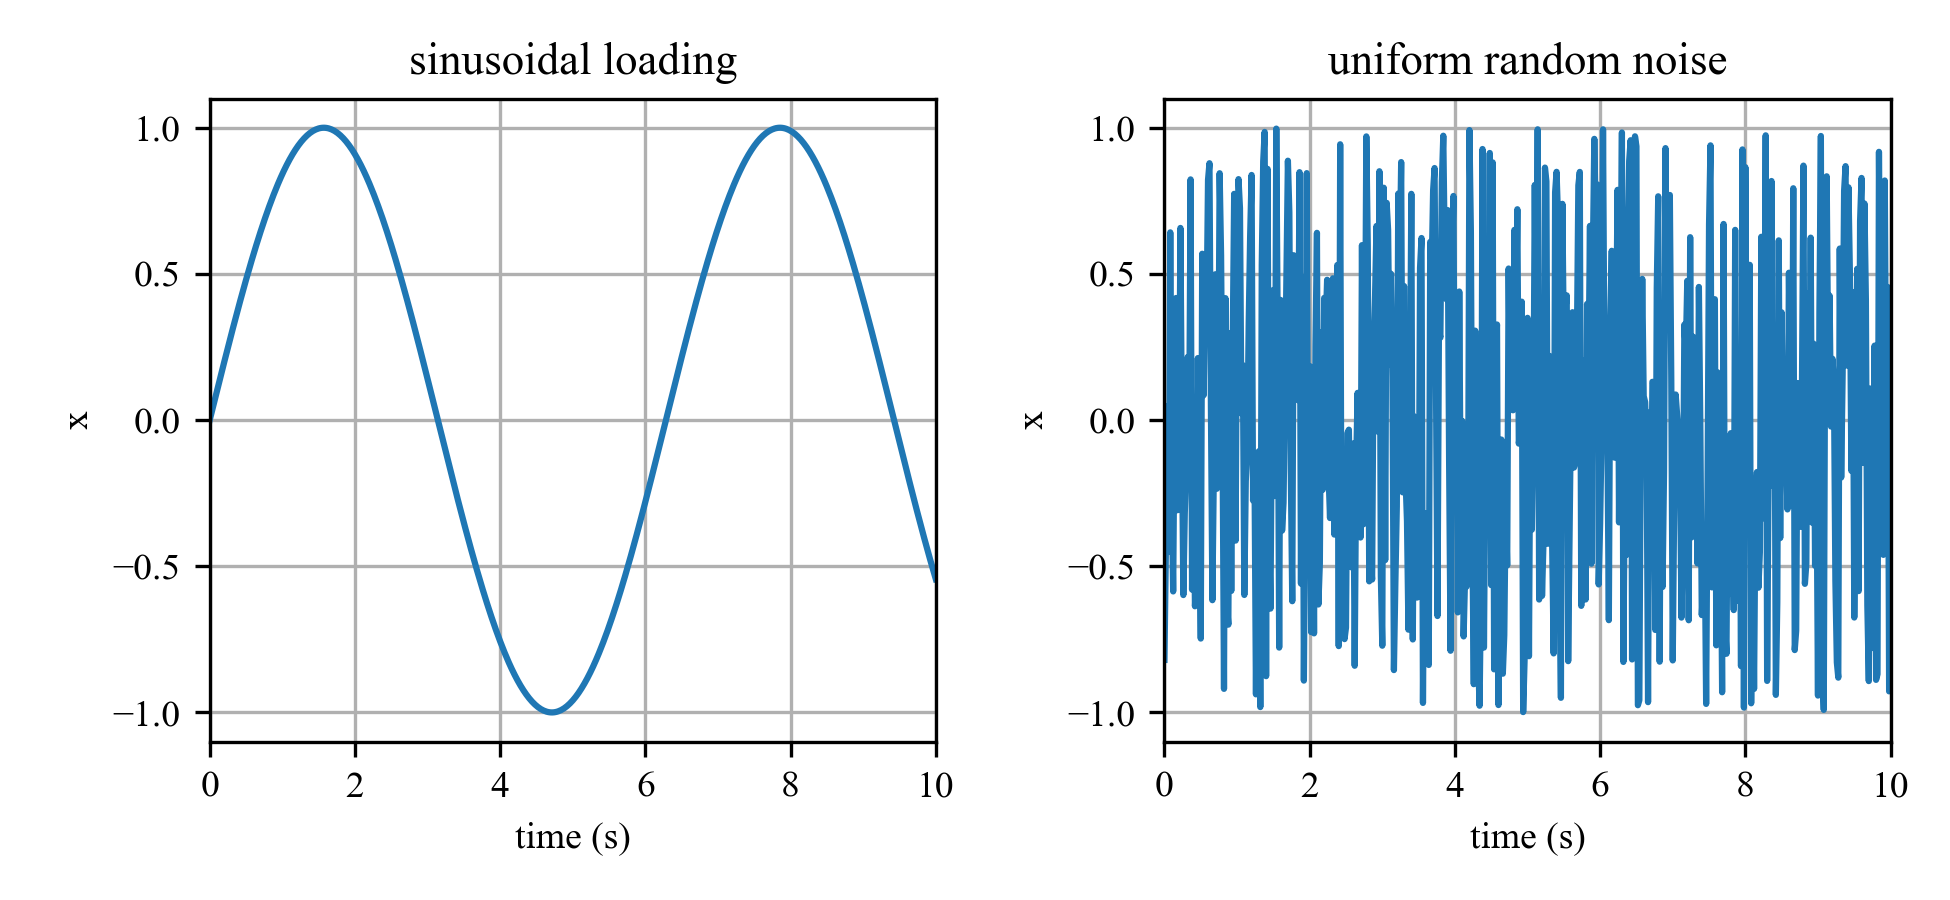
\includegraphics[width=1\textwidth]{../../Figures/Response_to_random_input_inputs.png}
\end{figure}

One of the fist factors to consider is the \textbf{mean of the random signal} $x(t)$, defined as:

\begin{equation}
E[x] = \bar{x} = \lim\limits_{T \rightarrow \infty} \frac{1}{T} \int_{0}^{T}x(t)dt
\end{equation}

where $T$ is the length in time of the data collected. However, for random signals we often want to consider signals with an average mean of zero (i.e. $\bar{x}(t)=0$). Therefore, for signals not centered around zero we can obtain a zero centered signal if the signal is stationary and we subtract the mean value from $\bar{x}$ from the signal $x(t)$. This can be written as:

\begin{equation}
x'(t) = x(t) - \bar{x}
\end{equation} 

where the $x'(t)$ is now centered around zero. As mentioned before, it is important to consider whether or not the input signals are stationary. A signal is \textbf{stationary} if its statistical properties (usually expressed by its mean) do not change with time. Here, it can be seen that for our inputs considered the signals are stationary if a long enough time period is considered. 

Another important variable is \textbf{variance} (or mean-square value) of the random variable $x(t)$ defined as:
\begin{equation}
E[x^2] = \bar{x^2} = \lim\limits_{T \rightarrow \infty} \frac{1}{T} \int_{0}^{T}x^2(t)dt
\end{equation}

and provides a measure of the magnitude of the fluctuations in the signal $x(t)$. This gives an easy way to calculate the root-mean-square (RMS) of the signal as:
\begin{equation}
x_\text{rms} = \sqrt{\bar{x^2}} 
\end{equation}

Now, considering the actual signal, a important measure of interests is how fast the value of the variables change. This is important to understand as it address how long it takes to measure enough samples of the variable before a meaningful statistical value can be calculated. One way to quantify how fast the values of signal change is the \textbf{autocorrelation function}: 
\begin{equation}
R_{xx}(\tau) = \lim\limits_{T \rightarrow \infty} \frac{1}{T} \int_{0}^{T}x(t)x(t+\tau)dt
\end{equation}
The subscript $xx$ denotes that this is a measure of the response for the variable xx, $\tau$ is the time difference between the values at which the signal $x(t)$ is sampled. The auto collation for the two inputs considered above are expressed below:
\begin{figure}[H]
	\centering
	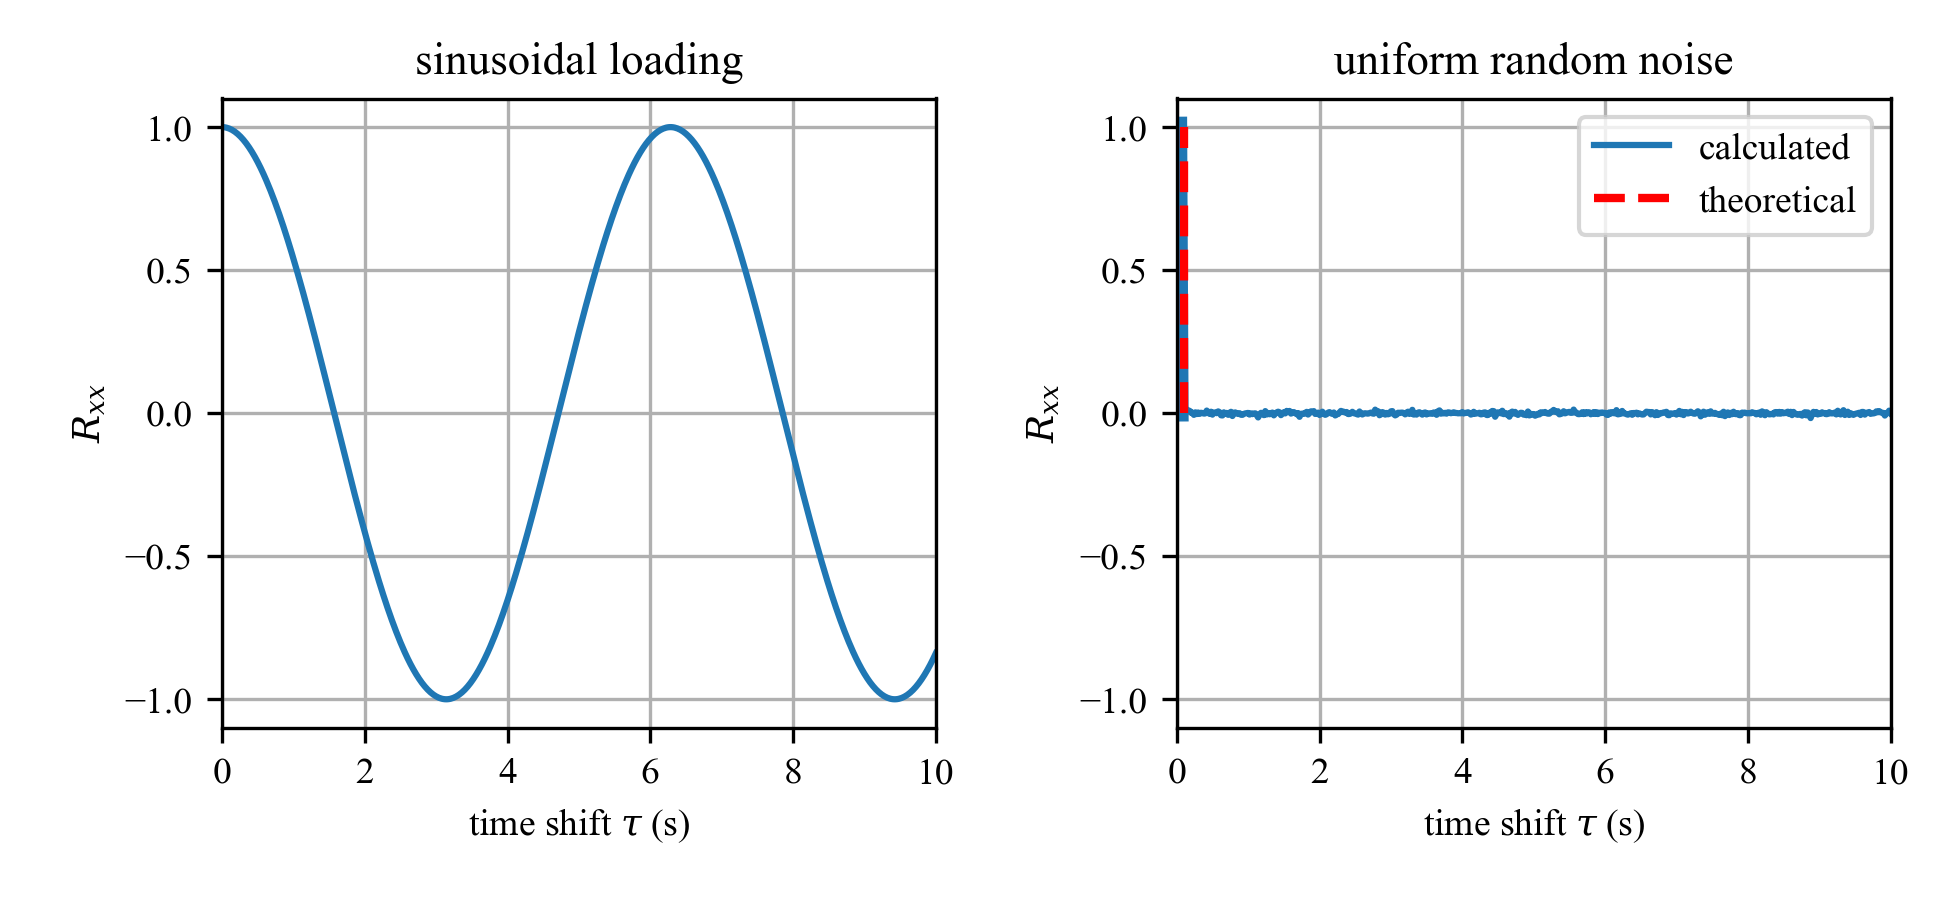
\includegraphics[width=1\textwidth]{../../Figures/Response_to_random_input_autocorrelation.png}
\end{figure}
Note that the value of $\tau$ selected in the auto correlation function greatly affects its response for the sinusoidal input. This is because the values for the sinusoidal are high correlated. To expand, the value at any time $t$ is greatly effected by the values immediately before and after it. This is not the case for the random input where the signal is not correlated and therefore there is little difference in changing the value of $\tau$ on the response of the autocorrelation function.  

Next, if we take the Fourier transform of the autocorrelation function we obtain the power spectral density (PSD) defined as:
\begin{equation}
S_{xx}(\omega) =\frac{1}{2 \pi} \int_{-\infty}^{\infty} R_{xx}(\tau) e^{-j \omega \tau}d \tau
\end{equation}
where the integral of $R_{xx}(\tau)$ changes the real number $\tau$ into the frequency-domain value $\omega$. The frequency spectrum (hence the $S$ in $S_{xx}(\omega)$) for the two input cases considered are plotted below.
\begin{figure}[H]
	\centering
	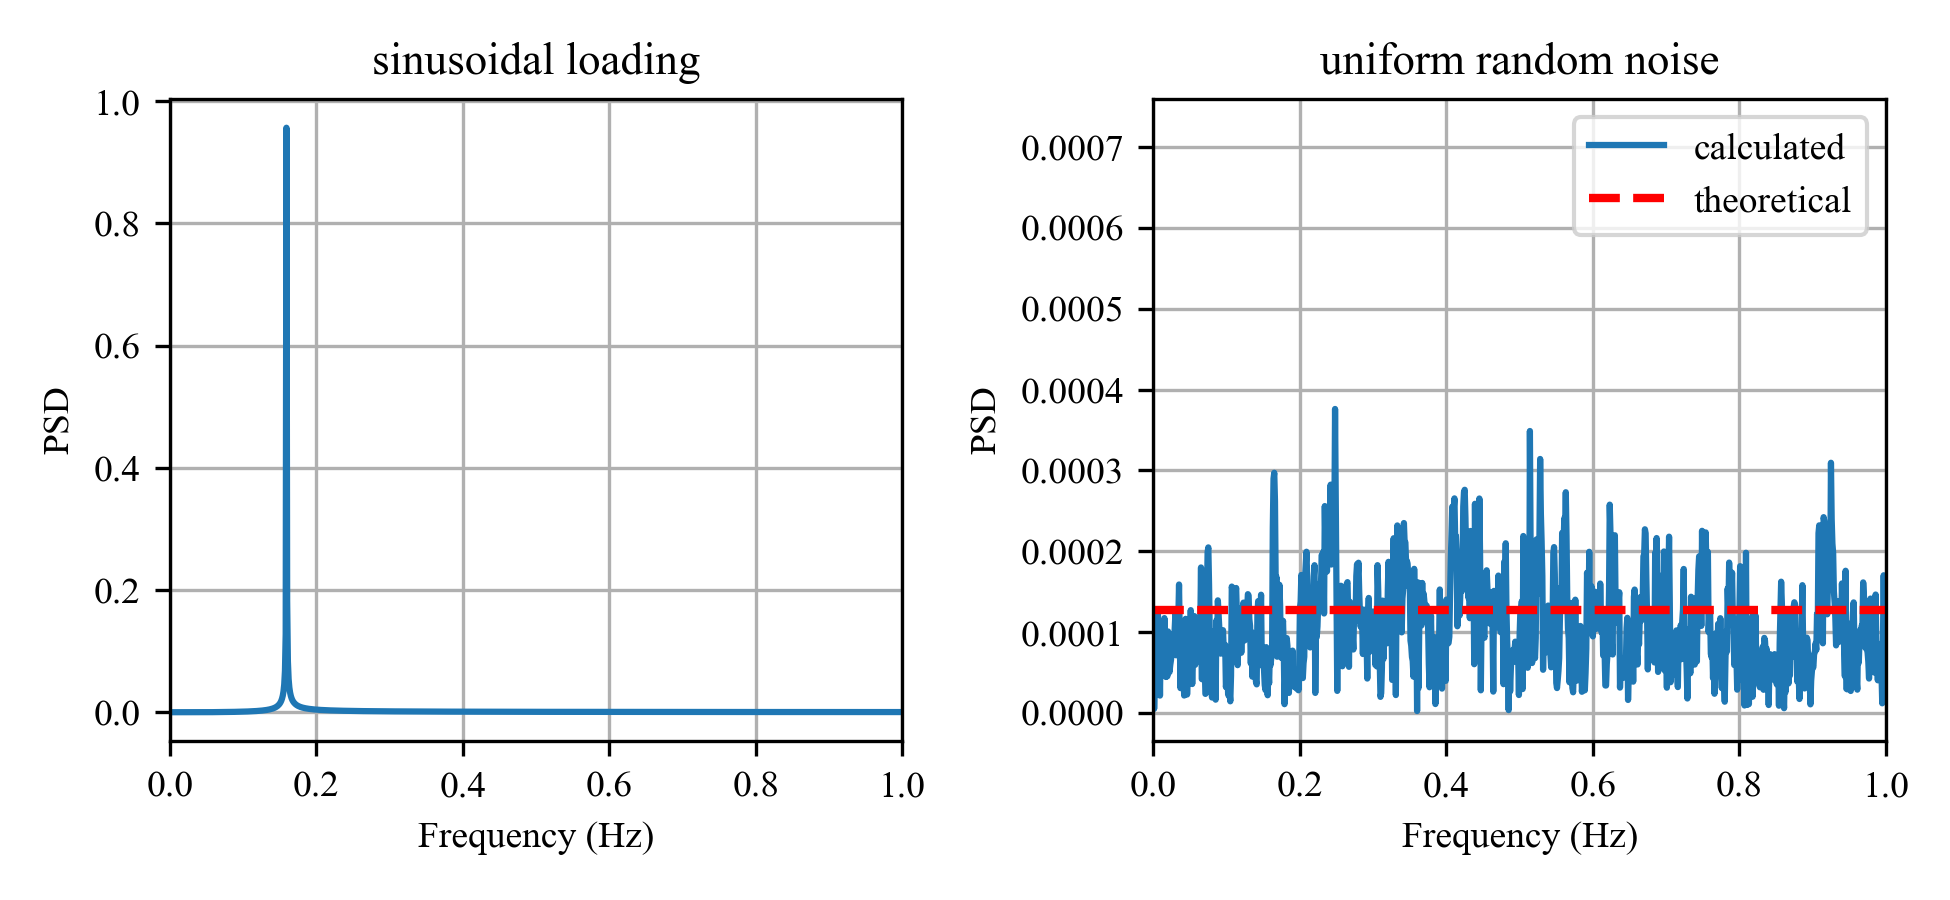
\includegraphics[width=1\textwidth]{../../Figures/Response_to_random_input_PSD.png}
\end{figure}
where the flat frequency response for the random input denotes that the random input is white noise input. A true white noise input would be perfectly flat, and is really just a theoretical concept. 

Recall that $S_{xx}$ is the spectrum of the response of the system. For the one-DOF system considered here, we can express an arbitrary input as a series of impulse inputs. 
\begin{figure}[H]
	\centering
	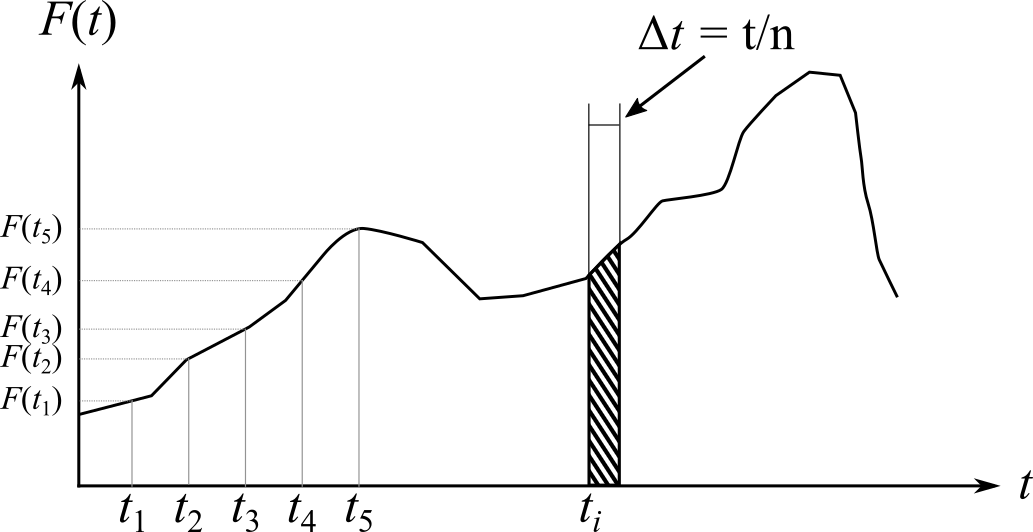
\includegraphics[width=0.7\textwidth]{../../Figures/Arbitary_excitation_forces.png}
\end{figure}
This knowledge, along with the frequency response function can be used to relate the spectrum of the input $S_{ff}(\omega)$ to the output through the transfer function as:
\begin{equation}
S_{xx}(\omega) =  |H(j\omega)|^2\Bigg[\frac{1}{2 \pi } \int_{-\infty}^{\infty} R_{ff}(\tau) e^{-j \omega \tau}d  \tau  \Bigg] 
\end{equation}
This can also be expressed in symbolic form as
\begin{equation}
S_{xx}(\omega) =  |H(j\omega)|^2 S_{ff}(\omega)
\end{equation}
where $R_{ff}$ denotes the autocorrelation function of $F(t)$ and $S_{ff}$ denotes the PSD of the forcing function $F(t)$. The notation $|H(j\omega)|^2$ is the square of the magnitude of the complex frequency response function. A more detailed derivation can be found in [Engineering Vibrations, Inman (2001)],[Random Vibrations, Spectral \& Wavelet Analysis, Newland (1993)], but here it is more important to study the results rather than the derivations. 

Another useful quantity to consider is the expected value of the output for a given input. The expected value $E[x]$, or $\bar{x}$, is expressed as:
\begin{equation}
E[x] =  \lim\limits_{T\rightarrow\infty} \int_{0}^{T} \frac{x(t)}{T}dt
\end{equation}
Additionally, the mean-square value can be directly related to the PSD function as 
\begin{equation}
E[x^2] = \bar{x^2} =   \int_{-\infty}^{\infty} |H(j\omega)|^2 S_{ff}(\omega) d\omega
\end{equation}
Moreover, for a constant input $S_{ff}(\omega) = S_0$ in therms of the frequency domain, the mean-square value can be expressed as:
\begin{equation}
E[x^2] = \bar{x^2} =   S_{0} \int_{-\infty}^{\infty} |H(j\omega)|^2 d\omega
\end{equation}

After inspecting the above equation, it becomes clear that to obtain the square of the expected value, a solution for  $\int_{-\infty}^{\infty} |H(j\omega)|^2$ must be obtained. For cases where $S_{ff}(\omega) = S_0$ and as such $S_{ff}(\omega)$ can be pulled out of the integral, these integrals have been solved [Random Vibrations, Spectral \& Wavelet Analysis, Newland (1993)]. For example, given $\int_{-\infty}^{\infty} |H(j\omega)|^2 d\omega$:

\begin{equation}
\int_{-\infty}^{\infty} \bigg|\frac{B_0}{A_0+j \omega A_1} \bigg|^2 d\omega = \frac{\pi B_0^2}{A_0 A_1}
\end{equation} 

and

\begin{equation}
\int_{-\infty}^{\infty} \bigg|\frac{B_0 + j \omega B_1}{A_0+j \omega A_1 - \omega^2 A_2} \bigg|^2 d\omega = \frac{\pi (A_0 B_1^2 + A_2 B_0^2)}{A_0 A_1 A_2}
\end{equation} 
When combined with the equation $E[x^2] = S_{0} \int_{-\infty}^{\infty} |H(j\omega)|^2 d\omega$, these integrals allow for the easy calculation of the expected values. 

\textbf{Example 1}

Considering the forced system:
\begin{figure}[H]
	\centering
	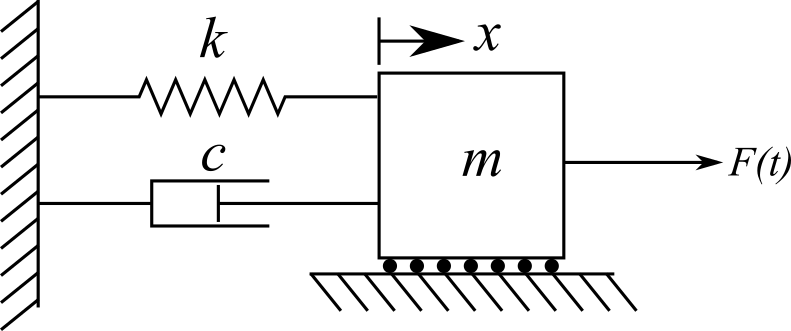
\includegraphics[width=0.4\textwidth]{../../Figures/forced_spring_mass_damper_system.png}
\end{figure}
Set the forcing function to be $F_0 \sin(\omega t)$ and calculate the transfer function. 

\textbf{Solution}

that can be expressed as the equation of motion
\begin{equation}
	m\ddot{x} + c\dot{x} +kx = F_0 \sin(\omega t)
\end{equation}
From the \#6 in the table for Laplace Transforms, we know that
\begin{equation}
	\Laplace{\sin(\omega t)} = \frac{\omega}{s^2+\omega^2}
\end{equation}
Therefore, 
\begin{equation}
F(s) = \frac{F_0\omega}{s^2+\omega^2}
\end{equation}
Ignoring the initial conditions and taking the Laplace transform of the EOM equation yields:
\begin{equation}
(ms^2 + cs +k)X(s) = \frac{F_0 \omega}{s^2+\omega^2} 
\end{equation}
Solving algebraically for the $X(s)$ yields: 
\begin{equation}
X(s) = \frac{F_0\omega}{(ms^2 + cs +k)(s^2+\omega^2)}
\end{equation}
Now that we have $F(s)$ and $X(s)$ we can obtain $H(s)$ as  
\begin{equation}
H(s) = \frac{X(s)}{F(s)} = \frac{F_0 \omega }{(ms^2 + cs +k)(s^2+\omega^2)} \cdot \frac{s^2+\omega^2}{F_0 \omega} = \frac{1}{ms^2+cs+k}
\end{equation}
or 
\begin{equation}
H(s) = \frac{1}{ms^2+cs+k}
\end{equation}
This is identical to the solution obtained using $F_0 \cos(\omega t)$ as would be expected because the transfer function is related to the system and not to the input. 

\textbf{Example 2}

Consider the following system

\begin{figure}[H]
	\centering
	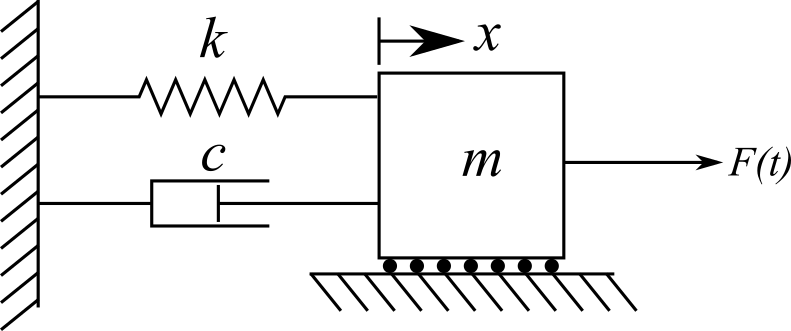
\includegraphics[width=0.4\textwidth]{../../Figures/forced_spring_mass_damper_system.png}
\end{figure}

Calculate the PSD of the response $x(t)$ given that the PSD of the applied force $S_{ff}(\omega)$ is white noise. 

\textbf{Solution}

From the system we know that the EOM is 

\begin{equation}
m\ddot{x} +c\dot{x} + kx = F(t)
\end{equation} 
The frequency response function for this system is 
\begin{eqnarray}
	H(j\omega) = \frac{1}{k-m\omega^2+c\omega j}
\end{eqnarray}
while the amplitude of the response is:
\begin{eqnarray}
H(\omega) = |H(j\omega)| = \frac{1}{\sqrt{(k-m\omega^2)^2+c^2\omega^2}}
\end{eqnarray}
Applying the equation that relates $S_{ff}(\omega)$ to $S_{xx}(\omega)$ we get:
\begin{equation}
S_{xx}(\omega) =  |H(j\omega)|^2 S_{ff}(\omega) = \bigg|\frac{1}{k-m\omega^2+c\omega j} \bigg|^2 S_{ff}(\omega) 
\end{equation}
White noise means the forcing function $S_{ff}(\omega)$ is constant across the frequency spectrum, therefore, $S_{ff}(\omega)=S_0$. Additionally as:
\begin{equation}
|H(j\omega)|^2 = \bigg|\frac{1}{k-m\omega^2+c\omega j} \bigg|^2 = \frac{1}{(k-m\omega^2)^2+c^2\omega^2}
\end{equation}
where the absolute value is the amplitude of the system. Therefore, we obtain:
\begin{equation}
S_{xx}(\omega) =  |H(j\omega)|^2 S_{0}= \frac{1}{(k-m\omega^2)^2+c^2\omega^2}S_0 = \frac{S_0}{(k-m\omega^2)^2+c^2\omega^2}
\end{equation}
Using various values for the elements in the system, the PSD for the system considered looks like:
\begin{figure}[H]
	\centering
	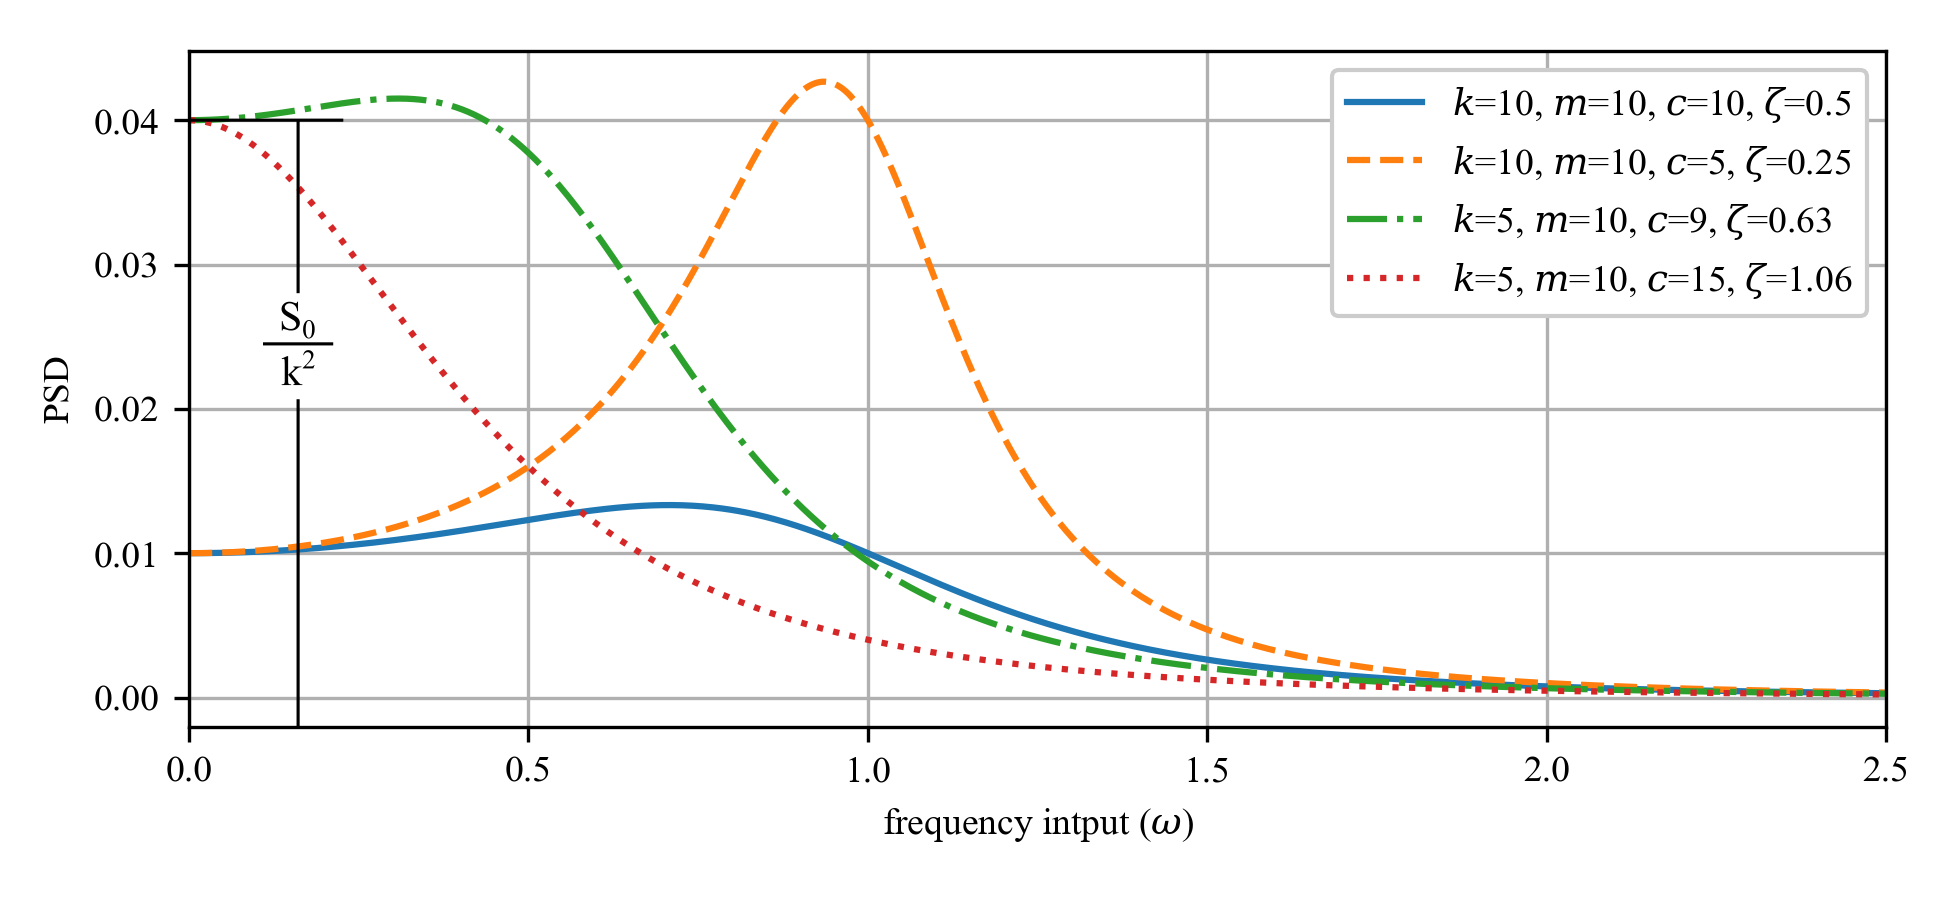
\includegraphics[width=1\textwidth]{../../Figures/response_to_white_noise_with_annotation.png}
\end{figure}

  



\textbf{Example 3}
For the same system as example 1, calculate the mean-square response of the system. 

\textbf{Solution}

Again, as the forcing function $S_{ff}(\omega)$ is constant across the frequency spectrum $S_{ff}(\omega)=S_0$ the mean-square response can be calculated as:
\begin{equation}
E[x^2] = \bar{x^2} =   S_{0} \int_{-\infty}^{\infty} |H(j\omega)|^2 d\omega
\end{equation}
Using the already tabulated response:
\begin{equation}
\int_{-\infty}^{\infty} \bigg|\frac{B_0 + j \omega B_1}{A_0+j \omega A_1 - \omega^2 A_2} \bigg|^2 d\omega = \frac{\pi (A_0 B_1^2 + A_2 B_0^2)}{A_0 A_1 A_2}
\end{equation} 
and the frequency response function:
\begin{equation}
H(j\omega) = \frac{1}{k-m\omega^2+c\omega j}
\end{equation}
when $B_0=1$, $B_1 = 0$, $A_0=k$, $A_1=c$, and $A_2 =m$. Therefore, using the tabulated expression we can show that:
\begin{equation}
E[x^2] = S_0 \frac{\pi m }{k c m} =  \frac{S_0 \pi}{k c}
\end{equation} 




\end{document}




















